\documentclass[12pt, oneside]{article}
\usepackage[letterpaper, margin=1in, headsep=0.5in, left=0.3in, right=2.5in]{geometry}
\usepackage[english]{babel}
\usepackage[utf8]{inputenc}
\usepackage{amsmath}
\usepackage{amsfonts}
\usepackage{amssymb}
\usepackage{tikz}
\usepackage{yhmath}
\usetikzlibrary{quotes, angles}
\usepackage{graphicx}
\usepackage{enumitem}
\usepackage{multicol}

\newif\ifmeta
\metatrue %print standards and topics tags

\title{Regents Geometry}
\author{Chris Huson}
\date{April 2022}

\usepackage{fancyhdr}
\pagestyle{fancy}
\fancyhf{}
\renewcommand{\headrulewidth}{0pt} % disable the underline of the header
\raggedbottom

%\fancyhead[LE]{\thepage}
\fancyhead[RO]{Name:}
\fancyhead[LO]{BECA / Dr. Huson / Geometry Regents Mixed Review}
\cfoot{\thepage}

\begin{document}
\subsubsection*{11.9 Linear equations}
\begin{enumerate}[itemsep=2cm]
\item The coordinates of the endpoints of directed line segment $PQR$ are $P(7,3)$ and $R(-5,7)$. If $PQ:QR = 1:3$, what are the coordinates of $Q$? \vspace{1.5cm}

\item A spherical glass float has a volume of $15,600$ cubic centimeters. What is the radius of the float to the nearest tenth of a centimeter? \vspace{1.5cm}

\item What is an equation of the image of the line $\displaystyle y=2x+6$ after a dilation with a scale factor of $\displaystyle \frac{3}{2}$ centered at the origin?

\item What are the coordinates of the center and the length of the radius of the circle whose equation is $(x+8)^2+(y-1)^2=100$? \vspace{1cm}

\item Which equation represents a line that is parallel to the line represented by\\[0.25cm] $\displaystyle y=\frac{3}{5}x+2$?
  \begin{multicols}{2}
    \begin{enumerate}
      \item $3x+5y=10$
      \item $3x-5y=15$ 
      \item $\displaystyle y=-\frac{3}{5}x+2$
      \item $\displaystyle y=-\frac{5}{3}x+4$
    \end{enumerate}
  \end{multicols}

\newpage
\item Two right triangles are shown below with $\angle A \cong \angle D$, $\angle C=33^\circ$, $BC=15$ cm, and $EF=10$ cm.
  \begin{center}
    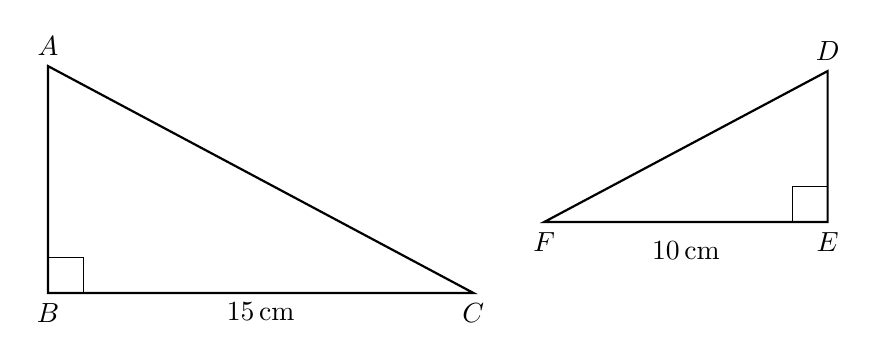
\begin{tikzpicture}[scale=0.9]
    \draw [thick]
      (0,0)node[below]{$F$}--
      (4,0)node[below]{$E$}--
      (4,2.13)node[above]{$D$}--cycle;
      \draw (4,0)++(-0.5,0)--++(0,0.5)--+(0.5,0);
    \draw [thick]
      (-1,-1)node[below]{$C$}--
      (-7,2.2)node[above]{$A$}--
      (-7,-1)node[below]{$B$}--cycle;
      \draw (-7,-1)++(0.5,0)--++(0,0.5)--+(-0.5,0);
      \node at (-4,-1)[below]{$15 \, \rm{cm}$};
      \node at (2,-0.4){$10 \, \rm{cm}$};
  \end{tikzpicture}
  \end{center}
Find $DF$, to the \emph{nearest tenth of a centimeter}. \vspace{2cm}

\item A regular pentagon is rotated about its center. Which degree measure will carry the regular pentagon onto itself? 
\begin{multicols}{2}
  \begin{enumerate}
    \item $45^\circ$
    \item $78^\circ$
    \item $120^\circ$
    \item $144^\circ$
  \end{enumerate}
\end{multicols}
  
\item The equation of a cirle is $x^2+y^2-2x+6y=54$. What are the center and radius of the circle?

\item Isosceles triangle $ABC$ is shown below with $AB=24$ and altitude $\overline{CD}$. If the area of $\triangle ABC$ is 60, find $BC$.
  \begin{center}
    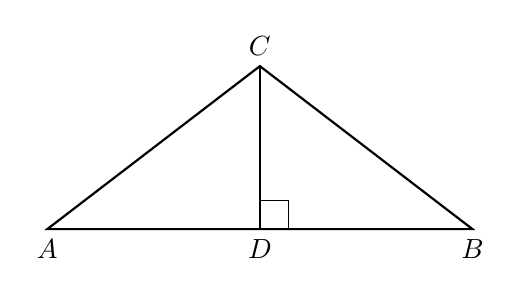
\begin{tikzpicture}[scale=0.9]
    \draw [thick]
    (0,0)node[below]{$A$}--
    (6,0)node[below]{$B$}--
    (3,2.3)node[above]{$C$}--cycle;
    \draw [thick](3,0)node[below]{$D$}--(3,2.3);
    \draw (3,0)++(0.4,0)--++(0,0.4)--+(-0.4,0);
  \end{tikzpicture}
  \end{center}

\end{enumerate}
\end{document}
  